\section{Матричный калькулятор}
\subsection{Условие задания}
Создать приложение,  реализующее основные операции с векторами и матрицами:

\begin{enumerate}
    \item Ввод матрицы, вектора;
    \item Создание матриц (единичная, матрица как набор векторов);
    \item Умножение на число, вектор, матрицу;
    \item Сложение/вычитание двух матриц;
    \item Сложение/вычитание двух векторов;
    \item Скалярное и векторное произведение двух векторов;
    \item Транспонированная матрица;
    \item Определитель, ранг матрицы.
\end{enumerate}

Выводить сообщения об ошибках (ввод не числа, несоответствие размерностей)

\subsection{Теория}
Вектором\cite{linal} называется направленный отрезок, для которого указаны его начало и конец. Свободный вектор --- множество одинаково направленных отрезков.

С точки зрения алгебры, вектор --- это строка или столбец матрицы.

Далее рассмотрим бинарные операции над векторами размерности $n \in \mathbb{N}$:
\begin{equation}
    \label{eq:vectors}
    \Vec{a} = \left(a_1, a_2, \dots, a_n\right),\;
    \Vec{b} = \left(b_1, b_2, \dots, b_n\right).
\end{equation}

Алгебраической суммой векторов (\ref{eq:vectors}) называют вектор:
\begin{equation}
    \Vec{a}+\Vec{b} = \left(a_1 + b_1, a_2 + b_2, \dots, a_n + b_n\right).
\end{equation}

Произведением вектора $\Vec{a}$ (\ref{eq:vectors}) на число $\lambda \in \mathbb{R}$ называют вектор:
\begin{equation}
    \lambda\Vec{a} = \left(\lambda a_1, \lambda a_2, \dots, \lambda a_n\right).
\end{equation}

Скалярным произведением векторов $\Vec{a} \cdot \Vec{b}$ (\ref{eq:vectors}) называют число:
\begin{equation}
    \Vec{a} \cdot \Vec{b} = \left|\Vec{a}\right|\left|\Vec{b}\right|\cos\angle\left(\Vec{a},\,\Vec{b}\right).
\end{equation}

Пусть $n = 3$ для векторов (\ref{eq:vectors}) --- из курса элементарной математики известно, что векторное произведение работает только в трёхмерном пространстве. Положим также, что векторы $\Vec{a}$ и $\Vec{b}$ не коллинеарны, то есть:
\begin{equation*}
    \exists\,i \in \mathbb{N}\cap\left[1,\,n\right]\;\forall\,\lambda\in\mathbb{N}\;a_i \neq \lambda b_i
\end{equation*}

Тогда векторным произведением называют вектор $\Vec{c}$ такой, что:
\begin{equation*}
    \begin{cases}
        \left|\Vec{c}\,\right| = S_{\Vec{a}\Vec{b}}, \\
        \Vec{c} \perp \Vec{a}, \\
        \Vec{c} \perp \Vec{b}, \\
        \left(\Vec{a},\,\Vec{b},\,\Vec{c}\right) - \textrm{правая тройка,}
    \end{cases}
\end{equation*}
где $S_{\Vec{a}\Vec{b}}$ --- площадь параллелограмма, построенного на $\Vec{a}$ и $\Vec{b}$ как на сторонах.

Матрицей называют прямоугольную таблицу чисел.

Далее рассмотрим матрицы:
\begin{equation}
    \label{eq:matrix}
    A = \begin{pmatrix} a_1^1 & \cdots & a_1^n \\ \vdots & \ddots & \vdots \\ a_n^1 & \cdots & a_n^n \\ \end{pmatrix},\;
    B = \begin{pmatrix} a_1^1 & \cdots & a_1^n \\ \vdots & \ddots & \vdots \\ a_m^1 & \cdots & a_m^n \\ \end{pmatrix},
\end{equation}
где $m,n\,\in\mathbb{N}$.

Матрицы вида $A$ (\ref{eq:matrix}) называют квадратными.

Пусть $i\,\in\mathbb{N}$ --- номер некоторой строки. Определителем квадратной матрицы называют число
\begin{equation}
    \left|A\right| = \det A = \begin{vmatrix} a_1^1 & \cdots & a_1^n \\ \vdots & \ddots & \vdots \\ a_n^1 & \cdots & a_n^n \\ \end{vmatrix}
    = \sum\limits_{k=1}^n\left(-1\right)^{k+i}a_i^kM_i^k,
\end{equation}
где $M_i^k$ -- определитель минора по элементу $A_i^k$. Это матрица, получаемая из исходной вычеркиванием строк и столбцов, содержащих $a_i^k$.

Определитель можно вычислить рекурсивно, сводя к базовому случаю $n=2$:
\begin{equation}
    \left|A\right| = \det A = \begin{vmatrix} a_1^1 & a_1^2 \\ a_2^1 & a_2^2 \\ \end{vmatrix}
    = a_1^1a_2^2 - a_1^2a_2^1,
\end{equation}

Ранг матрицы --- наивысший порядок среди порядков миноров этой матрицы, отличный от нуля. Вычисление ранга матрицы возможно методом Гаусса, что и было применено в программе.

Транспонированная матрица --- матрица со строками-столбцами и столбцами-строками исходной матрицы.

Алгебраическая сумма матриц определяется аналогичным векторам образом.

\subsection{Вид формы в конструкторе}
Форма имеет вид:

\begin{figure}
\centering
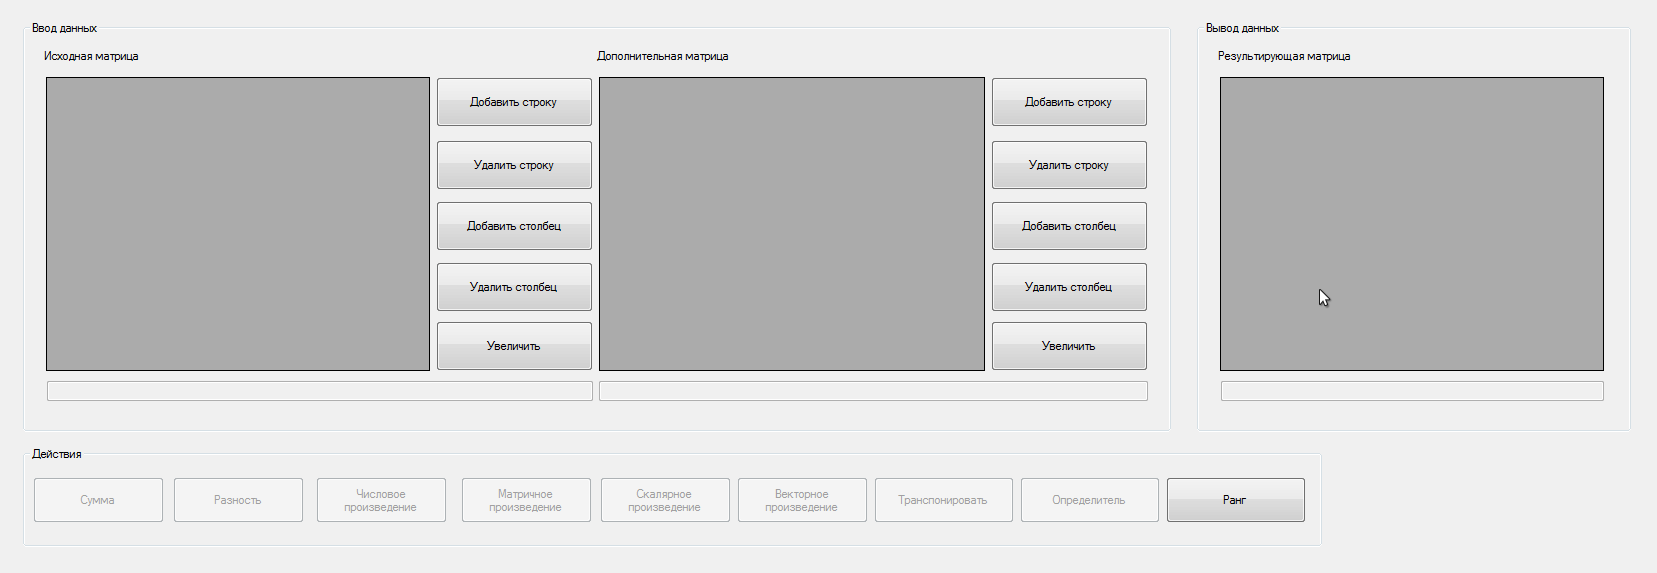
\includegraphics[width=0.5\linewidth]{images/matrix-calculator/form.png}
\caption{Форма окна для задания <<Простые вычисления>>}
\label{matrix-calculator-form}
\end{figure}

\subsection{Таблица с описанием элементов формы}
Все элементы формы были переименованы для большей читаемости. В таблице \ref{tab:matrix-calculator-form} представлены все изменения.


\begin{xltabular}{\textwidth}{| m{0.3\textwidth} | m{0.3\textwidth} | m{0.3\textwidth} |}

\hline
\textbf{Описание элементов формы} & \textbf{Список изменённых атрибутов} & \textbf{Новое значение атрибута} \\
\hline
\endfirsthead

\hline
\textbf{Описание элементов формы} & \textbf{Список изменённых атрибутов} & \textbf{Новое значение атрибута} \\
\hline
\endhead

\hline
\endfoot

\hline
\caption{Значение атрибутов элементов в матричном калькуляторе}
\label{tab:matrix-calculator-form}
\endlastfoot

Окно формы & Text & MatrixCalculator \\
Группа для ввода & Name & inputGroup \\
Группа для вывода & Name & outputGroup \\
Группа для действий & Name & actionsGroup \\
Метка для основной матрицы ввода & Name & initMatrixLabel \\
Метка для дополнительной матрицы ввода & Name & vectorLabel \\
Метка для матрицы вывода & Name & outputMatrixLabel \\
Таблица основной матрицы & Name & matrixInputInit \\
Таблица дополнительной матрицы & Name & matrixInputX \\
Таблица матрицы вывода & Name & matrixOutput \\
Поле ввода для вывода ошибок в исходной матрице & Name & inputInitErrorProvider \\
Поле ввода для вывода ошибок в дополнительной матрице & Name & inputXErrorProvider \\
Поле ввода для вывода ошибок в матрице вывода & Name & outputErrorProvider \\
Кнопка <<Добавить строку>> в исходную матрицу & Name & addRowInitButton \\
Кнопка <<Удалить строку>> в исходную матрицу & Name & rmRowInitButton \\
Кнопка <<Добавить столбец>> в исходную матрицу & Name & addColumnInitButton \\
Кнопка <<Удалить столбец>> в исходную матрицу & Name & rmColumnInitButton \\
Кнопка <<Увеличить>> в исходную матрицу & Name & addRowColumnInitButton \\
Кнопка <<Добавить строку>> в дополнительную матрицу & Name & addRowXButton \\
Кнопка <<Удалить строку>> в дополнительную матрицу & Name & rmRowXButton \\
Кнопка <<Добавить столбец>> в дополнительную матрицу & Name & addColumnXButton \\
Кнопка <<Удалить столбец>> в дополнительную матрицу & Name & rmColumnXButton \\
Кнопка <<Увеличить>> в дополнительную матрицу & Name & addRowColumnXButton \\
\end{xltabular}


\subsection{Примеры правильной и неправильной работы приложения}
При запуске приложения на экране появляется окно \ref{fig:matrix-calculator-start}.

\begin{figure}
\centering
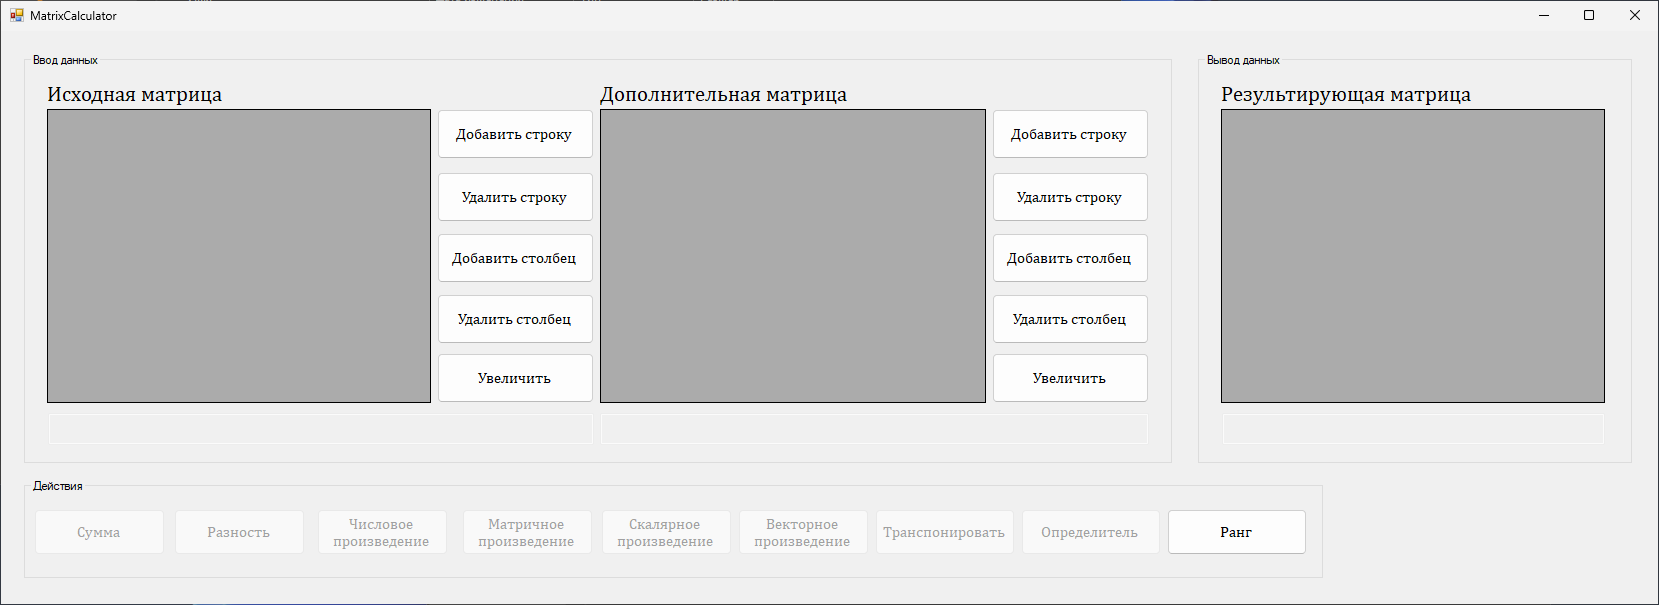
\includegraphics[width=0.5\linewidth]{images//matrix-calculator/start.png}
\caption{Запуск программы}
\label{fig:matrix-calculator-start}
\end{figure}

Кнопки активируются только тогда, когда операции над матрицами допустимы.\cite{patterny-oop} При нажатии на каждую кнопку происходит какое-то действие.

\begin{figure}
\centering
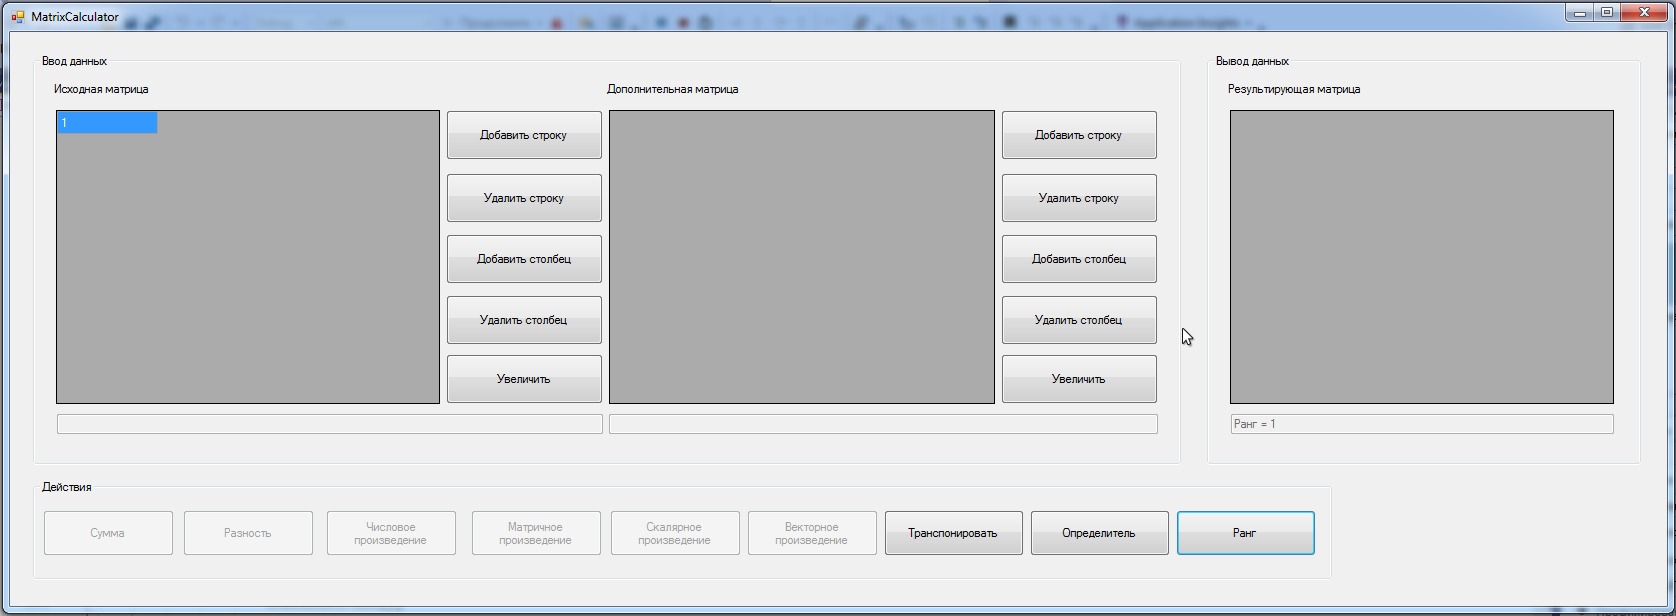
\includegraphics[width=0.5\linewidth]{images//matrix-calculator/okay.png}
\caption{Запуск с корректными данными}
\label{fig:matrix-calculator-okay}
\end{figure}

\begin{figure}
\centering
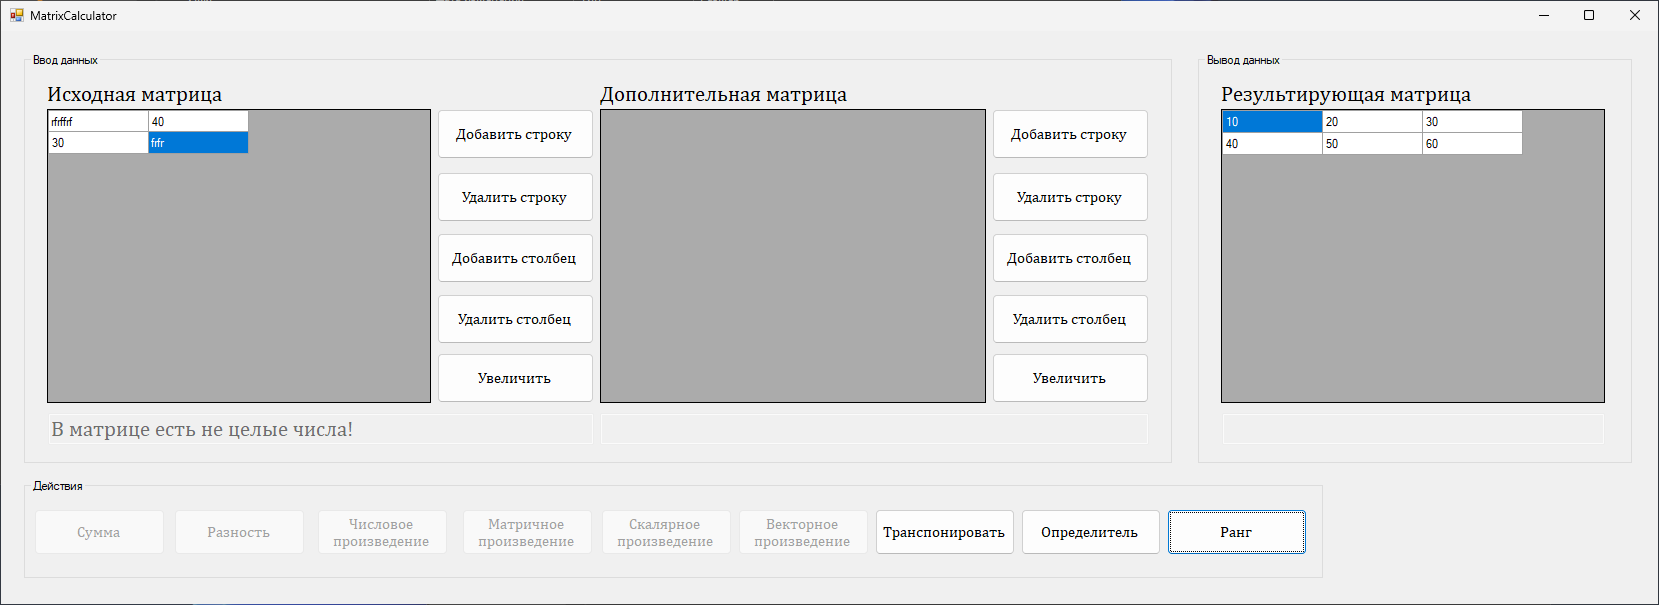
\includegraphics[width=0.5\linewidth]{images//matrix-calculator/error.png}
\caption{Пример ввода с некорректными данными}
\label{fig:matrix-calculator-error}
\end{figure}

\begin{figure}
\centering
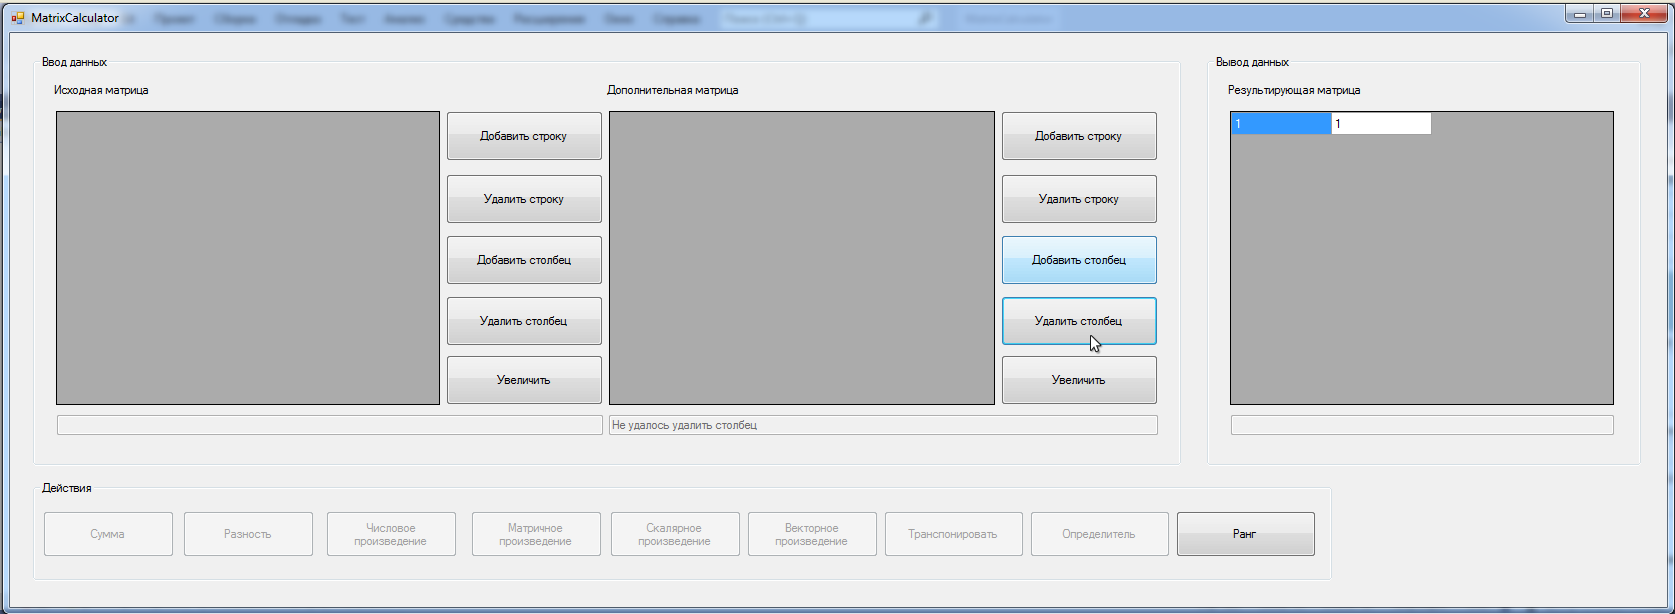
\includegraphics[width=0.5\linewidth]{images//matrix-calculator/error2.png}
\caption{Пример ввода с некорректными данными}
\label{fig:matrix-calculator-error2}
\end{figure}

\subsection{Примеры исходного кода}
\begin{minted}{cpp}
/* обработчик нажатия кнопки матричного произведения */
private: System::Void numericMultiplyButton_Click(System::Object^ sender, System::EventArgs^ e) {
    ClearAll();
    this->matrixOutput->RowCount = this->matrixInputInitial->RowCount;
    this->matrixOutput->ColumnCount = this->matrixInputInitial->ColumnCount;
    
    std::vector<std::vector<int>> matrixInitial;
    for (int i = 0; i < this->matrixInputInitial->RowCount; ++i) {
        std::vector<int> row;
        for (int j = 0; j < this->matrixInputInitial->ColumnCount; ++j) {
            int value;
            if (!Int32::TryParse(System::Convert::ToString(this->matrixInputInitial->Rows[matrixInputInitial->RowCount - i - 1]->Cells[j]->Value), value)) {
                this->inputInitialErrorProvider->Text = "В матрице есть не целые числа!";
                return;
            }
            row.push_back(value);
        }
    
        matrixInitial.push_back(row);
    }
    
    std::vector<std::vector<int>> matrixExtra;
    for (int i = 0; i < this->matrixInputExtra->RowCount; ++i) {
        std::vector<int> row;
        for (int j = 0; j < this->matrixInputExtra->ColumnCount; ++j) {
            int value;
            if (!Int32::TryParse(System::Convert::ToString(this->matrixInputExtra->Rows[matrixInputExtra->RowCount - i - 1]->Cells[j]->Value), value)) {
                this->inputExtraErrorProvider->Text = "В матрице есть не целые числа!";
                return;
            }
            row.push_back(value);
        }
    
        matrixExtra.push_back(row);
    }
    
    std::vector<std::vector<int>> matrixResult = multiplyMatrixByNumber(matrixInitial, matrixExtra[0][0]);
    
    for (int j = 0; j < this->matrixOutput->ColumnCount; ++j) {
        for (int i = 0; i < this->matrixOutput->RowCount; ++i) {
            this->matrixOutput->Rows[matrixInputInitial->RowCount - i - 1]->Cells[j]->Value = matrixResult[i][j];
        }
    }
}
\end{minted}

Больше кода проекта доступно в приложении \ref{application-A}. Также в приложенном архиве можно найти полный код проекта.